
%==========================================================================

\begin{frame}[fragile]

  {\Huge C++ Standard Algorithms}

  \vspace{10pt}

  {\large Kokkos implementation of a (growing set) of std algorithms}

  \vspace{20pt}

  \textbf{Objectives:}
  \begin{itemize}
  \item {Kokkos iterators}
  \item {Overview of supported algorithms}
  \item {Differences between the Kokkos and std API}
  \item {Examples}
  \item {Summary}
  \end{itemize}

  \vspace{-20pt}

\end{frame}

%==========================================================================

\begin{frame}[fragile]

  \begin{itemize}
  \item Iterators and std algorithms:
    \begin{itemize}
    \item Released with {\bf Kokkos 3.6}
    \item Include via header: \texttt{Kokkos\_StdAlgorithms.hpp}
    \end{itemize}
    \vspace{10pt}

  \item Inside the \texttt{Kokkos::Experimental}
    \begin{itemize}
    \item Please use them and send us feedback!
    \end{itemize}

    \vspace{10pt}
  \item Documentation is available in the Kokkos wiki:\\
    \url{https://github.com/kokkos/kokkos/wiki}

  \end{itemize}

\end{frame}

%==========================================================================

\begin{frame}[fragile]{Kokkos random-access iterators}

\textbf{\texttt{Kokkos::Experimental::\{begin, cbegin, end, cend\}}}

\vspace{10pt}
Declaration:
\begin{code}
template <class DataType, class... Properties>
KOKKOS_INLINE_FUNCTION
auto begin(const Kokkos::View<DataType, Properties...>& view);
\end{code}

\pause
\begin{itemize}
\item \texttt{view}: must be rank-1 with \texttt{LayoutLeft}, \texttt{LayoutRight},
  or \texttt{LayoutStride}.
\item Dereferencing iterators must be done in an execution space where `view` is accessible.
\end{itemize}

\pause
\vspace{5pt}
\texttt{Kokkos::Experimental::distance(first, last);}\\
\texttt{Kokkos::Experimental::iter\_swap(it1, it2);}

\end{frame}
%==========================================================================

\begin{frame}[fragile]{Algorithms: we use categories as in the C++ std}
  \begin{figure}
    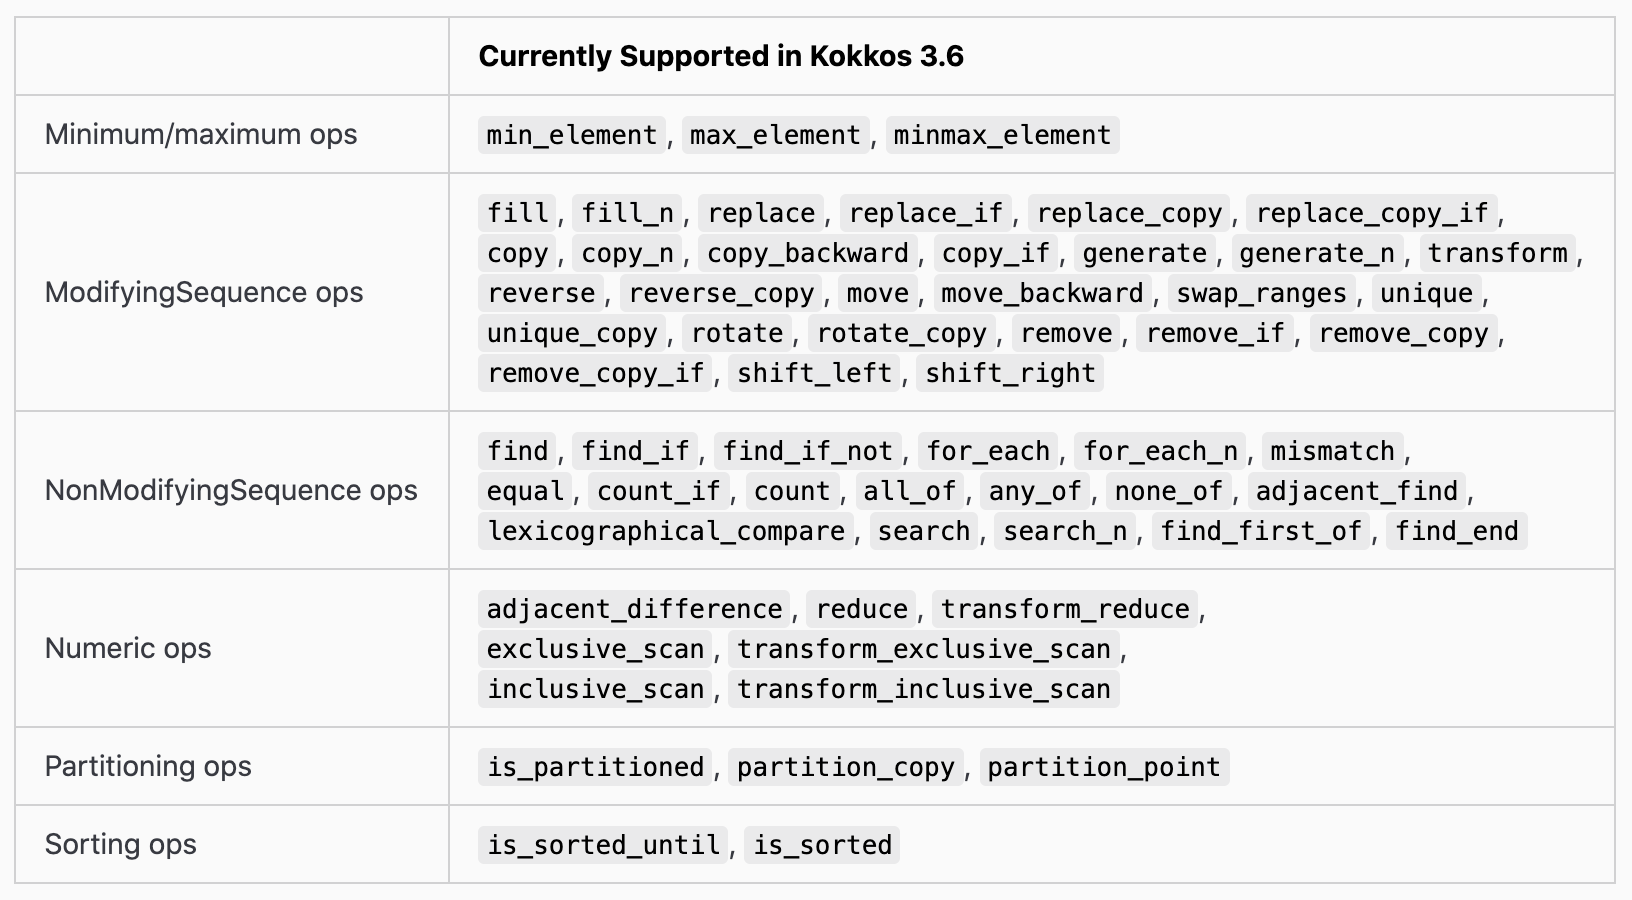
\includegraphics[width=1\linewidth]{algotable.png}
  \end{figure}

\end{frame}
%==========================================================================

\begin{frame}[fragile]{Algorithms: the key difference of our API}

- API accepting iterators:
\begin{code}
template <class ExeSpace, ...>
<return_type> algo_name(const ExeSpace& exespace, <iterators>);

template <class ExeSpace, ...>
<return_type> algo_name(const std::string& label,
                        const ExeSpace& exespace, <iterators>);
\end{code}

\vspace{10pt}
- API accepting Kokkos rank-1 views:
\begin{code}
template <class ExeSpace, ...>
<return_type> algo_name(const ExeSpace& exespace, <views>);

template <class ExeSpace, ...>
<return_type> algo_name(const std::string& label,
                        const ExeSpace& exespace, <views>);
\end{code}
\end{frame}
%==========================================================================

\begin{frame}[fragile]{Algorithms: the API details}

\begin{code}
template <class ExeSpace, ...>
<return_type> algo_name(const ExeSpace& exespace,   (1)
                        <iterators_or_views>);

template <class ExeSpace, ...>
<return_type> algo_name(const std::string& label,   (2)
                        const ExeSpace& exespace,
                        <iterators_or_views>);
\end{code}

\begin{itemize}
\item \texttt{exespace}: iterators/views MUST be accessible from it

\item \texttt{label}: passed to the implementation kernels for debugging
  \begin{itemize}
    \item For (1): ``Kokkos::algo\_name\_iterator\_api\_default'' or \\ \hspace{1.3cm}``Kokkos::algo\_name\_view\_api\_default''
  \end{itemize}

\item iterators: must be {\bf random access iterators}, preferably use \texttt{Kokkos::Experimental::begin,end,cbegin,cend}

\item views: rank-1, \texttt{LayoutLeft, LayoutRight, LayoutStride}
\end{itemize}

\end{frame}
%==========================================================================

\begin{frame}[fragile]{Algorithms: basic example}

  \hspace{-40pt}
  \begin{code}
    int main(){
      // ...
      namespace KE = Kokkos::Experimental;

      Kokkos::View<double*, Kokkos::HostSpace> myView("myView", 13);
      // assuming myView is filled somehow

      const double oldVal{2}, newVal{34};

      // act on the entire view
      KE::replace(Kokkos::DefaultHostExecutionSpace(),
                  KE::begin(myView), KE::end(myView), oldVal, newVal);

      // act on just a subset
      auto startAt = KE::begin(myView) + 4;
      auto endAt   = KE::begin(myView) + 10;
      KE::replace(Kokkos::DefaultHostExecutionSpace(), 
                  startAt, endAt, oldVal, newVal);

      // set label and execution space (assumed enabled)
      KE::replace("mylabel", Kokkos::OpenMP(),
                  myView, oldVal, newVal);
   }
  \end{code}
\end{frame}
%==========================================================================

\begin{frame}[fragile]{Algorithms: example with custom functor for comparison}

  \hspace{-40pt}
  \begin{code} %[basicstyle=\tiny]

     template <class ValueType1, class ValueType2 = ValueType1>
     struct CustomLessThanComparator {
       KOKKOS_INLINE_FUNCTION
       bool operator()(const ValueType1& a, const ValueType2& b) const
       {
        // here we use < but you can put any custom logic needed
        return a < b;
       }
     };

     int main(){
       // ...
       namespace KE = Kokkos::Experimental;
       Kokkos::View<double*, Kokkos::CudaSpace> myView("myView", 13);
       // fill a somehow
       auto res = KE::min_element(Kokkos::Cuda(), myView,
                                  CustomLessThanComparator<double>());
       //...
     }
  \end{code}
\end{frame}
%==========================================================================


\begin{frame}[fragile]{Algorithms: general considerations}

\begin{itemize}
\item Implementations rely on Kokkos parallel for, reduce or scan.

\vspace{10pt}
\item Debug mode enables several checks, e.g.: whether iterators
  identify a valid range, the execution space accessibility, etc.,
  and error messages printed.

\vspace{10pt}
\item If needed, algorithms fence directly the execution space instance provided:
  \hspace{-40pt}
  \begin{code}
    template <class ExeSpace, ...>
    <return_type> algo_name(const ExeSpace& exespace, ...)
    {
      // implementation
      exespace.fence(/*string depends on algorithm*/);
    }
  \end{code}
\end{itemize}

\end{frame}
%==========================================================================

\begin{frame}{Section Summary}

  \begin{minipage}{0.6\textwidth}
    \begin{itemize}
    \item Starting with Kokkos 3.6, Kokkos offers many std algorithms
      %\texttt{minimum/maximum, Numeric, ModifyingSequence, NonModifyingSequence, Partitioning, Sorting} ops
    \item Two main APIs: one for iterators and one for rank-1 views
    \item Checkout the documentation in the Kokkos wiki
    \end{itemize}
  \end{minipage}
  \begin{minipage}{0.38\textwidth}
    \begin{figure}
      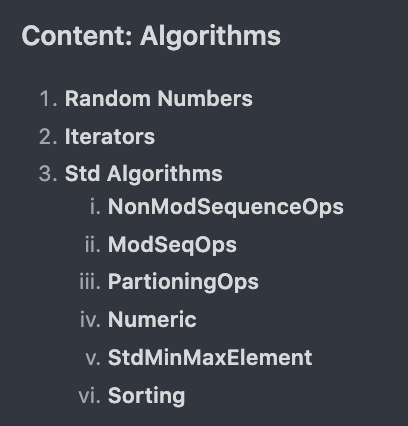
\includegraphics[width=0.7\linewidth]{algowiki.png}
      \caption{Wiki documentation}
    \end{figure}
  \end{minipage}

  \begin{itemize}
  \item{Useful to make your code more expressive, allowing us to worry about having performant implementations}
  \item{Please use them, and let us know of any issues!}
  \item{Try them with the new feature: \texttt{Kokkos::Experimental::partition\_space}}
  \item{In progress: team-level implementations}
  \end{itemize}

\end{frame}
